%! Author = leo
%! Date = 25.07.20

% Preamble
\documentclass{beamer}
\usetheme{metropolis}
\usepackage[backend=bibtex,style=numeric]{biblatex}
\addbibresource{literature.bib}
\setbeamertemplate{bibliography item}{\insertbiblabel}

% Packages
\usepackage{amsmath}
\usepackage{amssymb}
\usepackage{bm}
\usepackage{mathtools}
\usepackage{booktabs}
\usepackage{tabularx}

% Commands
\DeclarePairedDelimiterX{\infdivx}[2]{(}{)}{%
#1\;\delimsize\|\;#2%
}
\newcommand{\kldiv}{D_{KL}\infdivx}

\title{Semantic Representations in Variational Autoencoders as a Model of the Visual System}
\subtitle{Master Thesis Presentation}
\author{Leonard Papenmeier}
\date{\today}

% Document
\begin{document}
    \maketitle
    \begin{frame}{Outline}
        \tableofcontents
    \end{frame}


    \section{Introduction}
    \begin{frame}{Biological Plausibility}
        \begin{columns}
            \begin{column}{0.48\textwidth}
                Supervised CNNs have shown relatedness to the Visual System:
                \begin{itemize}
                    \item Emergence of Gabor wavelets~\cite{krizhevsky2012imagenet}
                    \item Explanation of IT activity~\cite{khaligh2014deep}
                \end{itemize}
            \end{column}
            \begin{column}{0.48\textwidth}
                \begin{figure}
                    \centering
                    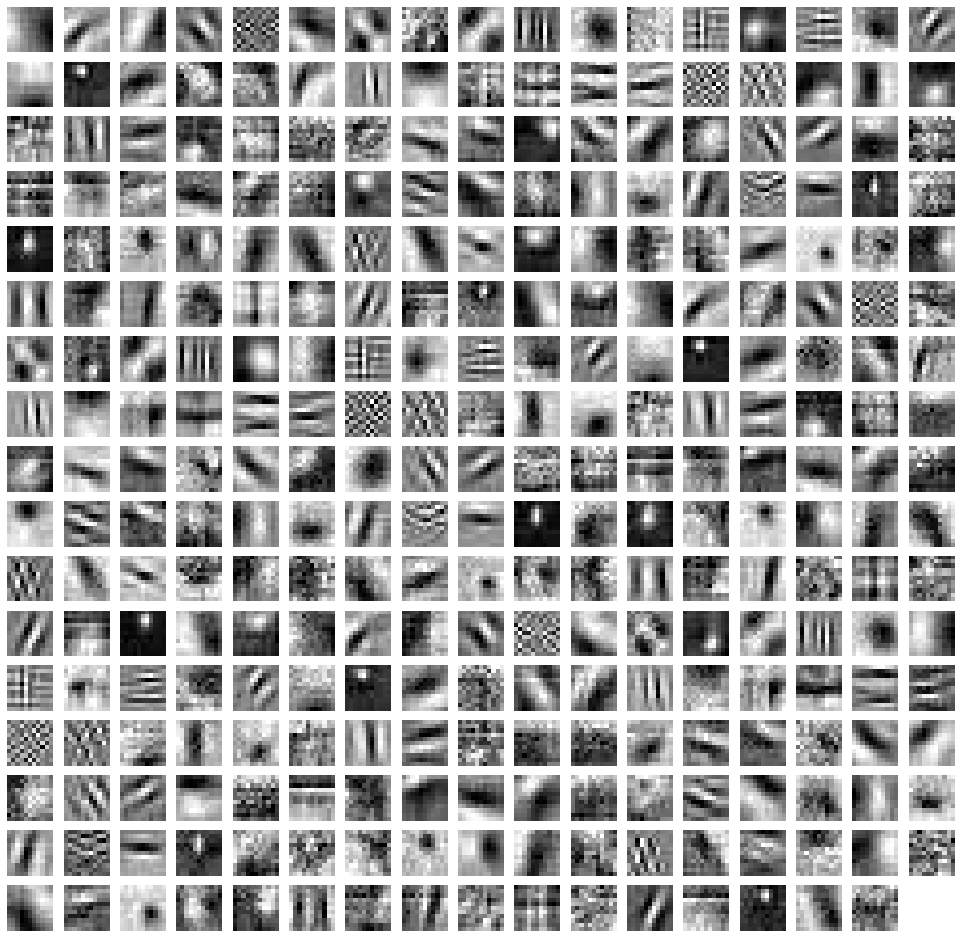
\includegraphics[width=\textwidth]{images/alexnet_classification_l1_kernels.png}
                    \caption{Gabor Wavelets in the first Layer of AlexNet~\cite{krizhevsky2012imagenet}}
                    \label{fig:figure_gabor}
                \end{figure}
            \end{column}
        \end{columns}
    \end{frame}
    \begin{frame}{Variational Autoencoder (VAE)}
        \begin{columns}
            \begin{column}{0.48\textwidth}
                \begin{itemize}
                    \item Requires no labeled data
                    \item Allows sampling of latent space
                    \item Topographic map
                    \item Latent space arithmetic
                \end{itemize}
            \end{column}
            \begin{column}{0.48\textwidth}
                \begin{figure}
                    \centering
                    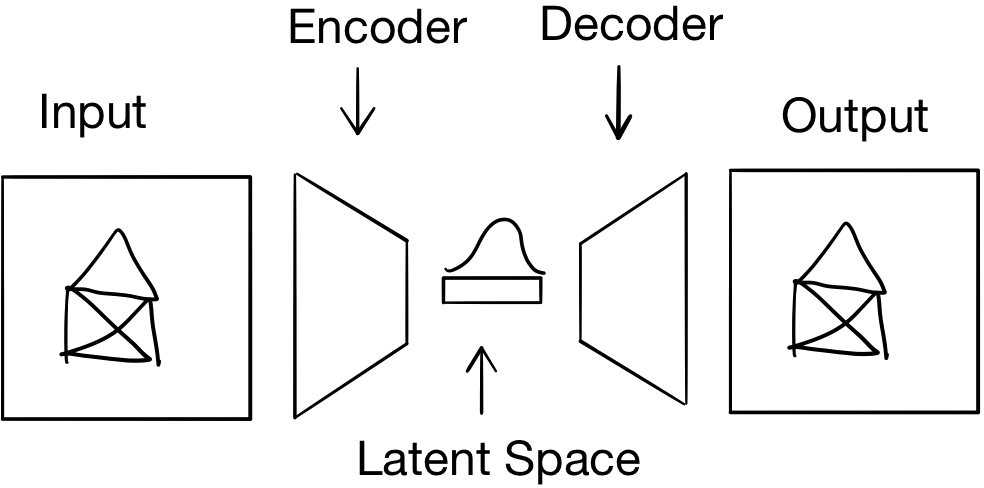
\includegraphics[width=\textwidth]{pres_imgs/vae_sketch.png}
                    \caption{Abstract Visualization of a VAE}
                    \label{fig:vae_sketch}
                \end{figure}
            \end{column}
        \end{columns}
    \end{frame}
    \begin{frame}{The Variational Autoencoder as a Model of the Visual System}
        The controllable latent space and the general biological plausibility of CNNs make the VAE an interesting candidate of a model of the visual system.
    \end{frame}


    \section{Theoretical Background}
    \begin{frame}{The Human Visual System}
        \begin{columns}
            \begin{column}{0.48\textwidth}
                The Visual Cortex is mainly hierarchically structured.
                The ventral pathway encodes the \textit{what}, the dorsal pathway the \textit{where}~\cite{goodale1992separate}.

                \begin{itemize}
                    \item Simple and complex cells
                    \item Sparse coding
                \end{itemize}
            \end{column}
            \begin{column}{0.48\textwidth}
                \begin{figure}
                    \centering
                    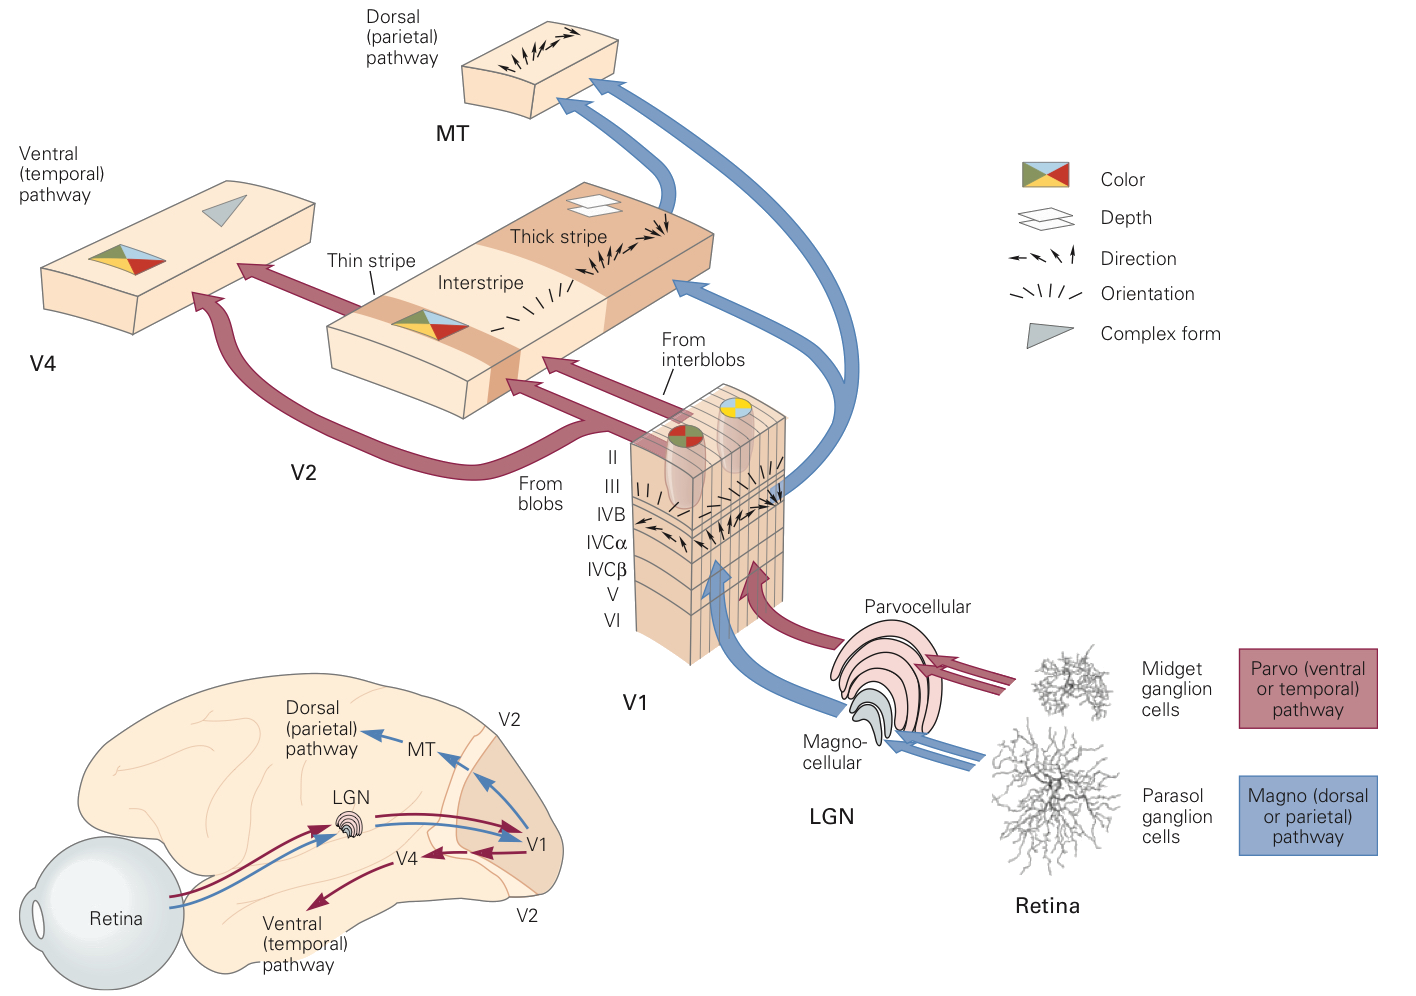
\includegraphics[width=\textwidth]{pres_imgs/ventral_dorsal.png}
                    \caption{Hierarchical structure of the Visual Cortex, and Ventral and Dorsal Pathways (taken from \cite[p. 571]{mack2013principles})}
                    \label{fig:figure_ventral_dorsal}
                \end{figure}
            \end{column}
        \end{columns}
    \end{frame}
    \begin{frame}{Convolutional Neural Networks}
        \begin{columns}
            \begin{column}{0.48\textwidth}
                Convolutions are models of S-cells~\cite{lindsay2020convolutional}.

                A subsequent down-scaling introduces translation invariance (C-cells)~\cite{lindsay2020convolutional}.
            \end{column}
            \begin{column}{0.48\textwidth}
                \begin{figure}
                    \centering
                    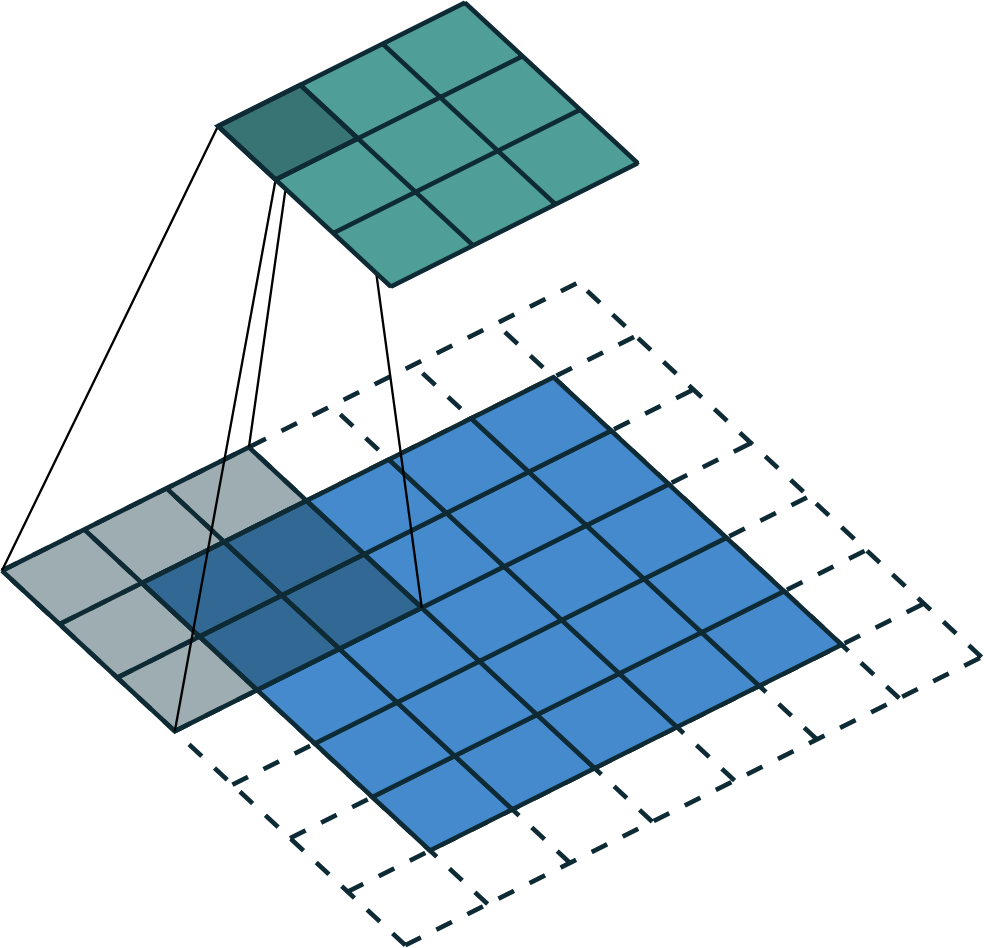
\includegraphics[width=\textwidth]{pres_imgs/convolution_example.png}
                    \caption{Example of a convolution, taken from \cite{dumoulin2016guide}}
                    \label{fig:example_convolution}
                \end{figure}
            \end{column}
        \end{columns}
    \end{frame}
    \begin{frame}{Variational Autoencoders 1}
        A VAE has two spaces: $\bm{z}$- and $\bm{x}$-space.
        The model learns a joint probability distribution.
        \begin{align*}
            p(\bm{x}) &= \int p(\bm{x}, \bm{z})d\bm{z}\\
            &= \int p(\bm{x}|\bm{z})\,p(\bm{z})d\bm{z}.
        \end{align*}
    \end{frame}
    \begin{frame}{Variational Autoencoders 2}
        Given $\bm{x}$, what is the latent space distribution?
        \begin{align*}
            p(\bm{z}|\bm{x}) &= \frac{p(\bm{x}|\bm{z})p(\bm{z})}{p(\bm{x})} \\
            p(\bm{x}) &= \int p(\bm{x}|\bm{z})p(\bm{z})d\bm{z}
        \end{align*}
        Computing the posterior $p(\bm{z}|\bm{x})$ is intractable!
    \end{frame}
    \begin{frame}{Variational Autoencoders 3}
        \begin{columns}
            \begin{column}{0.48\textwidth}
                The \textit{true} posterior $p(\bm{z}|\bm{x})$ is approximated by an \textit{inference model} $q_\phi(\bm{z}|\bm{x})$.

                VAEs minimize the difference between the true and the approximated posterior.
            \end{column}
            \begin{column}{0.48\textwidth}
                \begin{figure}
                    \centering
                    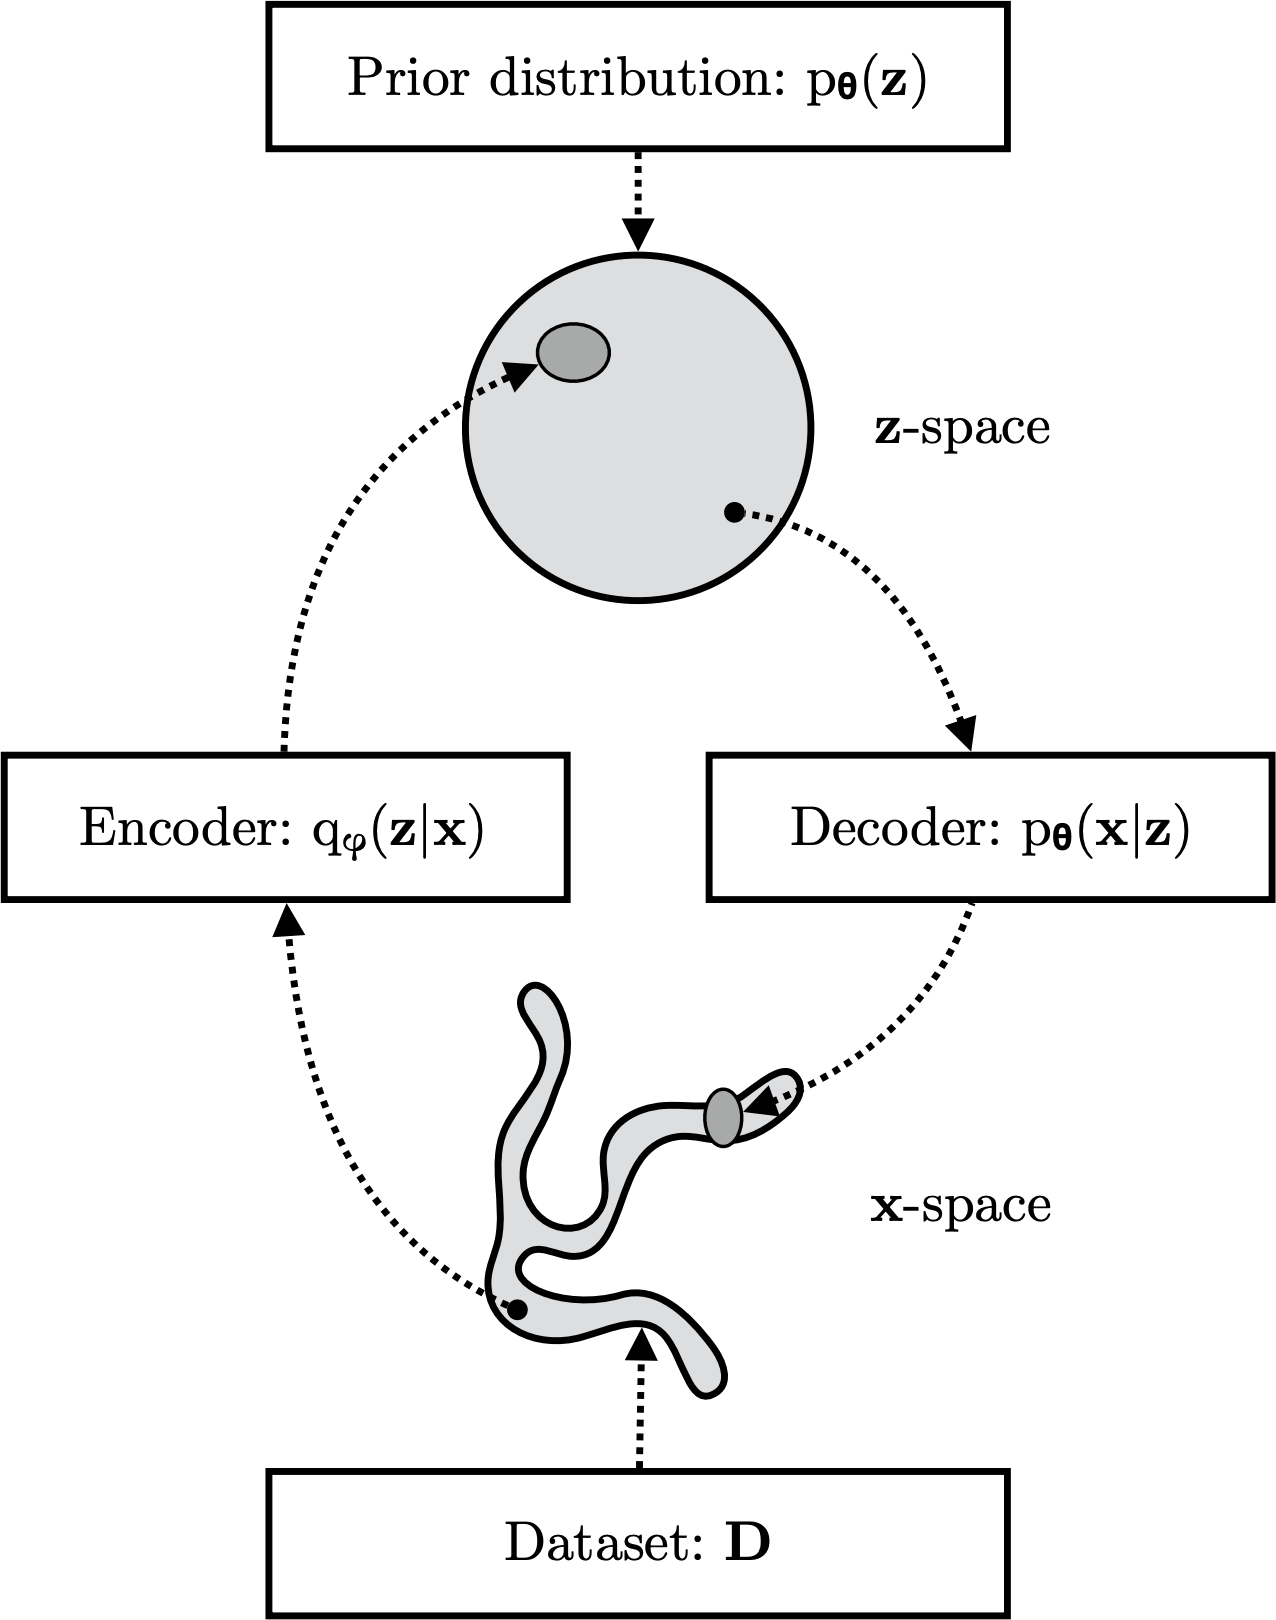
\includegraphics[width=.9\textwidth]{pres_imgs/vae_interplay.png}
                    \caption{Data and latent distributions in VAEs, taken from~\cite{kingma2019introduction}}
                    \label{fig:vae_interplay}
                \end{figure}
            \end{column}
        \end{columns}
    \end{frame}
    \begin{frame}{VAE Training Objective 1}
        \begin{align*}
            \kldiv{q_\phi(\bm{z}|\bm{x})}{p_\theta(\bm{z}|\bm{x})} &= -\sum_{\bm{z}} q_\phi(\bm{z}|\bm{x}) \log \frac{p_\theta(\bm{z}|\bm{x})}{q_\phi(\bm{z}|\bm{x})} \\
            &= \ldots \\
            &= -\sum_{\bm{z}} q_\phi(\bm{z}|\bm{x}) \log \frac{p_\theta(\bm{x},\bm{z})}{q_\phi(\bm{z}|\bm{x})} + \log p_\theta(\bm{x})
        \end{align*}
        Then
        \begin{align*}
            \underbrace{\vphantom{\sum_{\bm{z}} x}\log p_\theta(\bm{x})}_{\text{constant}} =  \underbrace{\vphantom{\sum_{\bm{z}} x}\kldiv{q_\phi(\bm{z}|\bm{x})}{p_\theta(\bm{z}|\bm{x})}}_{\downarrow}  + \underbrace{\sum_{\bm{z}} q_\phi(\bm{z}|\bm{x}) \log \frac{p_\theta(\bm{x},\bm{z})}{q_\phi(\bm{z}|\bm{x})}}_{\uparrow}.
        \end{align*}
    \end{frame}
    \begin{frame}{VAE Training Objective 2}
        \begin{align*}
            \sum_{\bm{z}} q_\phi(\bm{z}|\bm{x}) \log \frac{p_\theta(\bm{x},\bm{z})}{q_\phi(\bm{z}|\bm{x})} &= \sum_{\bm{z}} q_\phi(\bm{z}|\bm{x}) \log \frac{p_\theta(\bm{x}|\bm{z})p_\theta(\bm{z})}{q_\phi(\bm{z}|\bm{x})}\\
            &= \sum_{\bm{z}} q_\phi(\bm{z}|\bm{x}) \left[ \log p_\theta(\bm{x}|\bm{z}) + \log \frac{p_\theta(\bm{z})}{q_\phi(\bm{z}|\bm{x})} \right]\\
            &= \underbrace{\sum_{\bm{z}} q_\phi(\bm{z}|\bm{x})\log p_\theta(\bm{x}|\bm{z})}_{=\mathbb{E}_{q_\phi(\bm{z}|\bm{x})}\left[ \log p_\theta(\bm{x}|\bm{z}) \right]} + \underbrace{\sum_{\bm{z}} q_\phi(\bm{z}|\bm{x})\log \frac{p_\theta(\bm{z})}{q_\phi(\bm{z}|\bm{x})}}_{=\kldiv{q_\phi(\bm{z}|\bm{x})}{p_\theta(\bm{z})}}. \label{eq:elbo_error_term}
        \end{align*}
    \end{frame}
    \begin{frame}{VAE Training Objective 3}
        \begin{columns}
            \begin{column}{0.48\textwidth}
                $\mathbb{E}_{q_\phi(\bm{z}|\bm{x})}\left[ \log p_\theta(\bm{x}|\bm{z}) \right]$ is basically the mean squared error between input and output.

                The KL-term has a simple closed form if $q_\phi(\bm{z}|\bm{x})$ is independent and $p(\bm{z})$ chosen to be standard normal.
            \end{column}
            \begin{column}{0.48\textwidth}
                \begin{figure}
                    \centering
                    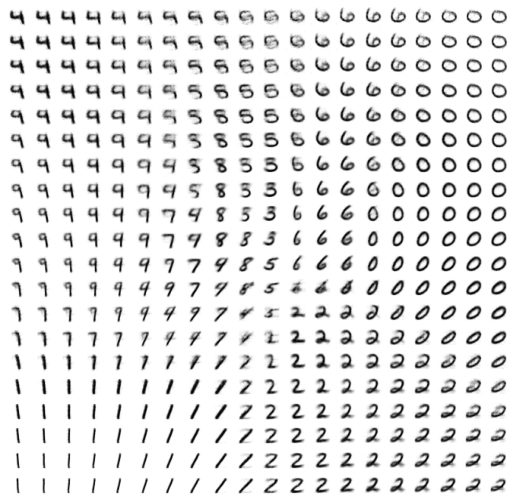
\includegraphics[width=\textwidth]{images/latent_space_traversals/vae_mnist.png}
                    \caption{Latent Space Exploration of a VAE on Hand-Written Digits}
                    \label{fig:vae_mnist}
                \end{figure}
            \end{column}
        \end{columns}
    \end{frame}
    \begin{frame}{Variational Ladder Autoencoder 1}
        \begin{columns}
            \begin{column}{0.48\textwidth}
                Employ multiple latent spaces $\bm{z}_i$ with inference networks of differing capacities.
            \end{column}
            \begin{column}{0.48\textwidth}
                \begin{figure}
                    \centering
                    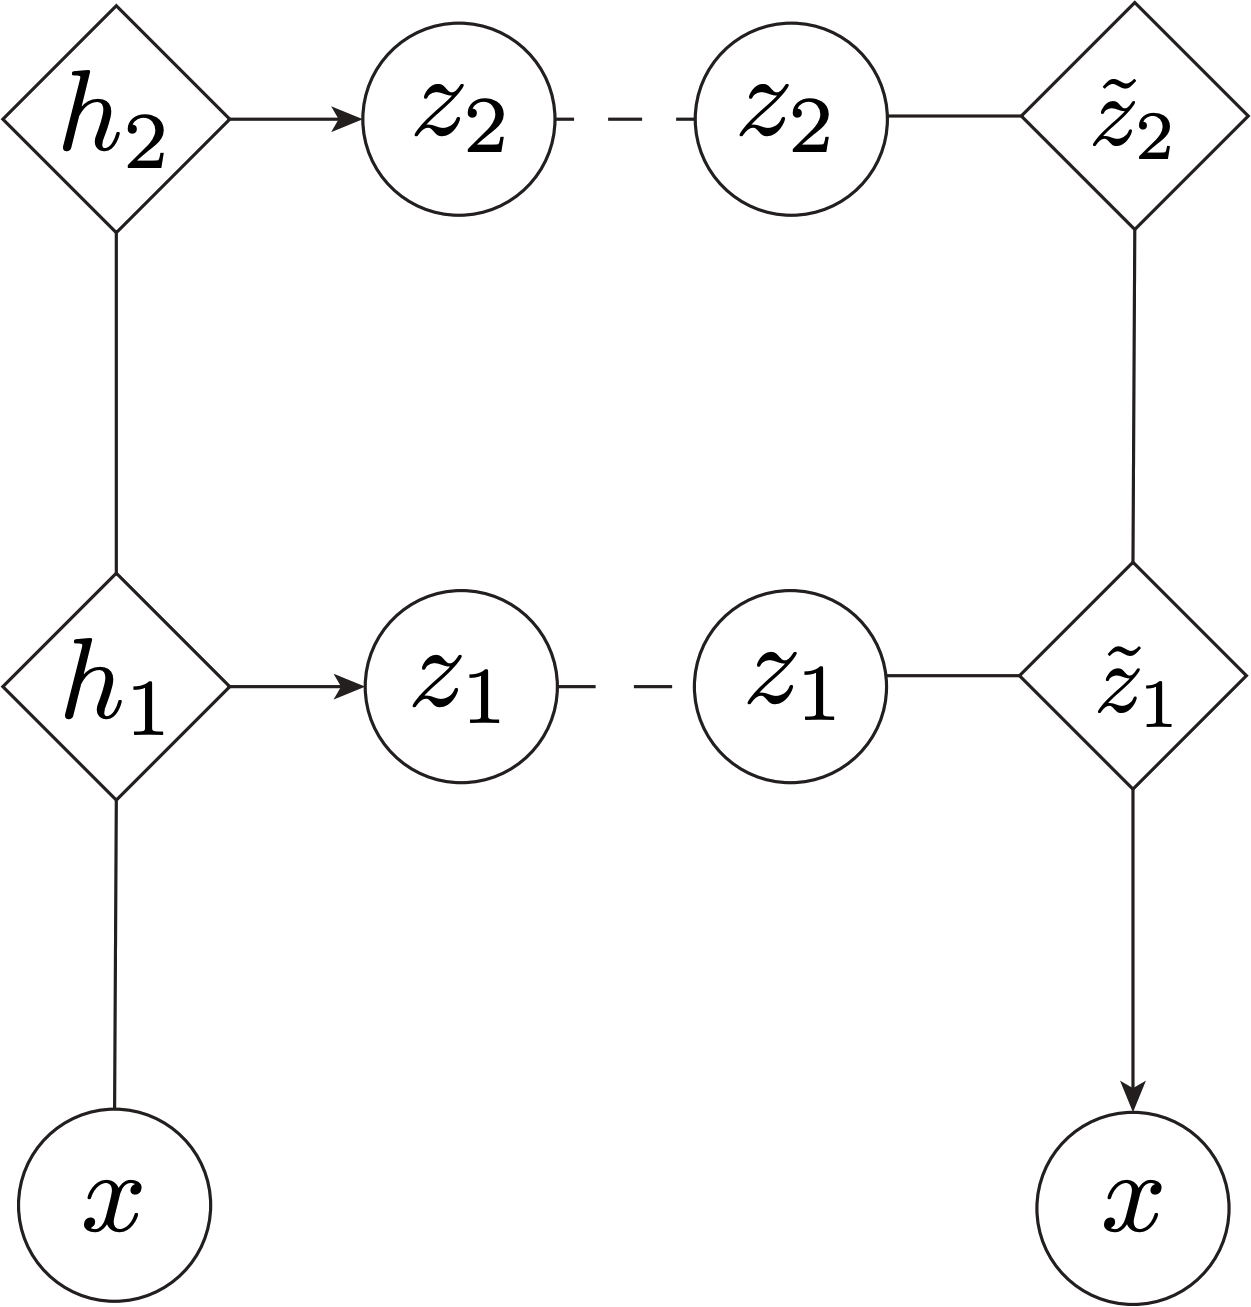
\includegraphics[width=\textwidth]{pres_imgs/vlae_structure.png}
                    \caption{VLAE Structure, taken from~\cite{zhao2017learning}}
                    \label{fig:vae_structure}
                \end{figure}
            \end{column}
        \end{columns}
    \end{frame}
    \begin{frame}{Variational Ladder Autoencoder 2}
        \begin{columns}
            \begin{column}{0.3\textwidth}
                Layers with a less powerful inference network learn lower-level factors of variation.
            \end{column}
            \begin{column}{0.68\textwidth}
                \begin{figure}
                    \centering
                    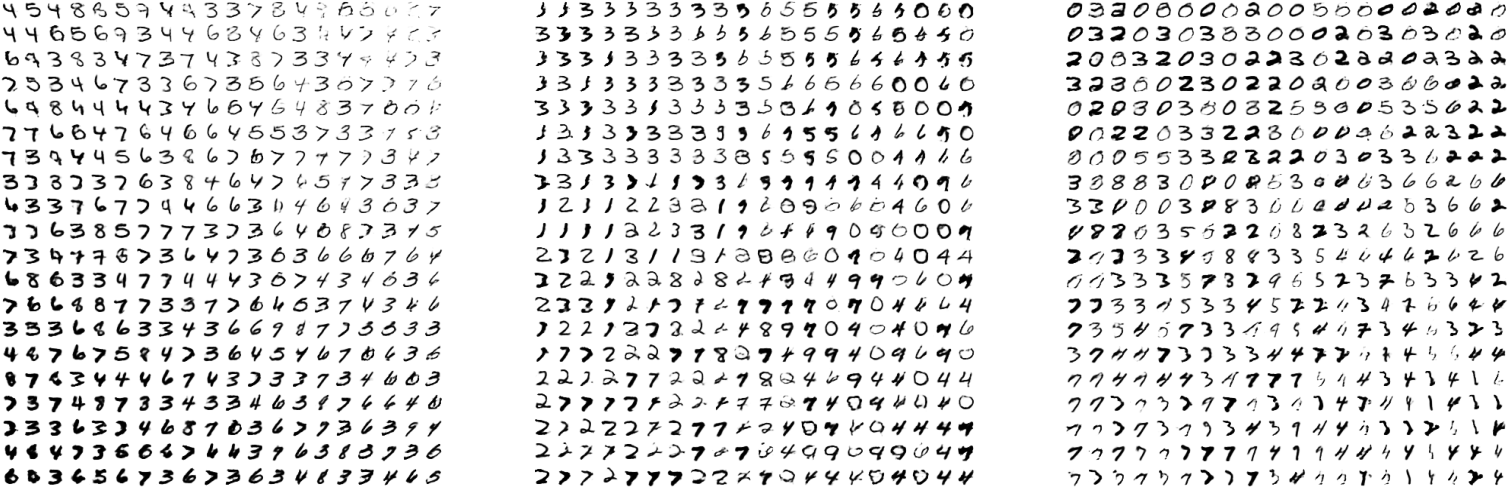
\includegraphics[width=\textwidth]{images/latent_space_traversals/vlae_mnist.png}
                    \caption{Latent Space Exploration of a 3-Layer VLAE on Hand-Written Digits}
                    \label{fig:vlae_mnist}
                \end{figure}
            \end{column}
        \end{columns}
    \end{frame}
    \begin{frame}{Latent Space Disentanglement / Separability}
        \begin{enumerate}
            \item Changing one factor of variation affects only \ldots
            \begin{itemize}
                \item \ldots a single (linear) subspace in the latent space (\textit{Disentanglement}).
                \item \ldots a single layer $\bm{z}_i$ (\textit{Separability}).
            \end{itemize}
            \item Generating $\bm{\tilde{x}}$ by sampling from $\bm{z}$ approximately leads to the data distribution.
        \end{enumerate}
    \end{frame}


    \section{Methods}
    \begin{frame}{Research Questions 1}
        \begin{table}[H]
            \begin{tabularx}{\textwidth}{llX}
                \toprule \\
                \multicolumn{2}{l}{Number} & Question \\
                \midrule \\
                RQ1 &    & Are VAEs or VLAEs related to the visual cortex in terms of \ldots                                      \\
                & a) & \hspace{1cm} \ldots the emergence of Gabor wavelets?                                                   \\
                & b) & \hspace{1cm} \ldots sparse coding?                                                                     \\
                RQ2 &    & Do VAEs or VLAEs fulfil the requirements of latent space disentanglement or latent space separability? \\
                RQ3 &    & Can VAEs or VLAEs represent both continuous and categorical factors of variation in the latent space?  \\
                RQ4 &    & How do VAEs and VLAEs represent lower factors of variation in the latent space?                        \\
            \end{tabularx}
        \end{table}
    \end{frame}
    \begin{frame}{Research Questions 2}
        \begin{table}[H]
            \begin{tabularx}{\textwidth}{llX}
                RQ5 & & Do VAEs or VLAEs learn independent factors of variation independently in the latent space?              \\
                RQ6 & & Are the latent spaces of VLAEs independent in terms of generated images?                                \\
                RQ7 & & Do VAE/VLAE-generated images resemble the data distribution?                                            \\
                RQ8 & & Is the discriminative loss superior to the pixel-wise loss in terms of the previous research questions? \\
                \bottomrule
            \end{tabularx}
            \caption{Research Questions}
        \end{table}
    \end{frame}
    \section*{References}
    \begin{frame}[allowframebreaks]{References}
        \printbibliography
    \end{frame}
\end{document}